\section{Конструкторский раздел}

В конструкторском разделе разработан метод программной реализации доверенной среды исполнения с помощью виртуализации процессоров архитектуры ARM и представлено его формализованное описание в виде диаграмм IDEF0 и схем алгоритмов. Выполнено проектирование ПО для реализации данного метода.

\subsection{Проектирование метода программной реализации доверенной среды исполнения}

Разработанный метод предполагает использование принципа разделения функциональности на разные компоненты системы. Система спроектирована таким образом, что при атаке или получении доступа к одному из компонентов, её целостность нарушена не будет. Для корректной работы метода, система обязательно должна поддерживать технологию ARM TrustZone и аппаратные механизмы виртуализации ARM.

Каждой гостевой виртуальной машине сопоставляется виртуальная машина выполняющая роль доверенной среды исполнения, для достижения данной цели используется гипервизор. Каждая из этих виртуальных машин выполняется в обычном мире.

Для обеспечения целостности и проверки последовательности загрузки используется безопасный мир (который является частью ARM TrustZone). В безопасном мире располагаются модули отображения адресов памяти гипервизора и виртуальных машин; модуль перехода и сохранения контекста между виртуальными машинами. Такой подход обеспечивает целостность данных, даже если код гипервизора был скомпрометирован.

Каждая ДСИ использует своё индивидуальное рабочее окружение, в котором хранятся данные. Окружение закреплено за конкретной виртуальной машиной и доступное только когда процессор выполняется в режиме hypervisor, с помощью чего и добивается изоляция. При этом, само окружение не является частью сущности гипервизора.

Для корректного и безопасного взаимодействия вышеописанных компонентов: модулей расположенных в безопасном мире, рабочих окружений и виртуальных машин используется модуль блокировки потока управления, который является частью гипервизора.

На рисунке \ref{fig:full-design} представлена диаграмма компонентов системы для разработанного метода программной реализации ДСИ.

\begin{figure}[h]
	\centering
	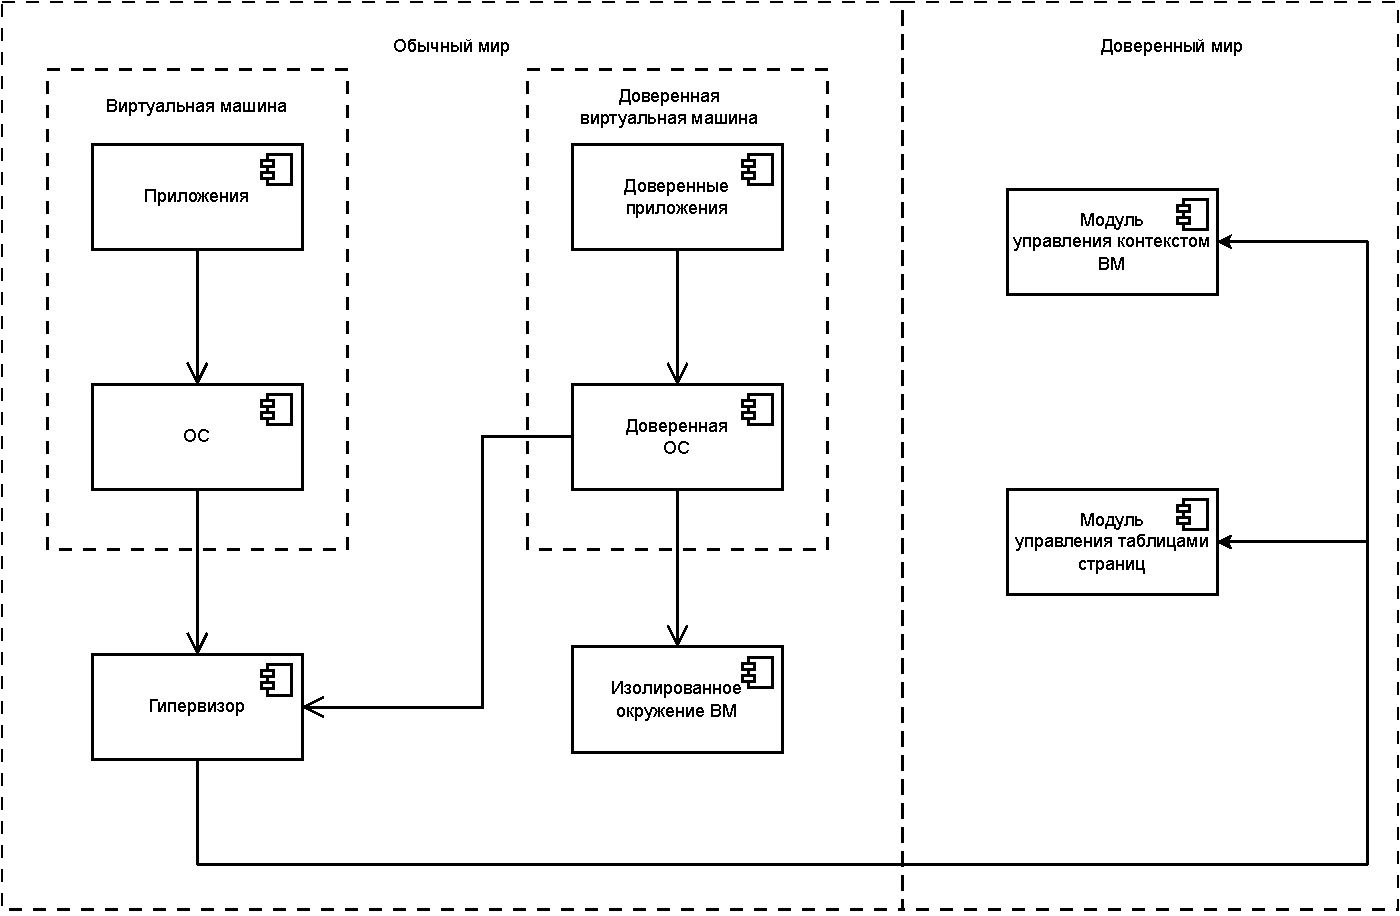
\includegraphics[width=\textwidth]{img/design-diagram-of-components.pdf}
	\caption{Диаграмма компонентов системы}
	\label{fig:full-design}
\end{figure}

Далее будет дано детальное описание разрабатываемых модулей и окружений.

\subsubsection{Модуль защищенного отображения памяти}

Модуль отображения памяти отвечает за трансляцию виртуальных адресов в физические в режиме выполнения hypervisor, а так же промежуточных виртуальных в физические для гостевых виртуальных машин. Модуль выполняется в безопасном мире и предоставляет два интерфейса для гипервизора, которые позволяют загрузить и модифицировать таблицу страниц.

Система построена таким образом, что модуль отображения памяти обладает монопольным доступом к загрузке и модификации таблицы страниц. Это достигается с помощью допущений, описанных ниже.

\begin{itemize}
	\item [---] Гипервизор не может изменять регистр, в котором хранится указатель на таблицу страниц: все инструкции, позволяющие это сделать, удаляются из его исходного кода. Сами страницы памяти, на которых располагаются таблицы страниц, помечаются как только для чтения для гипервизора.
	\item [---] Страницы памяти, на которых расположен код гипервизора, помечаются как только для чтения. Это позволяет гарантировать что исходный код не может быть изменен во время исполнения.
	\item [---] После запуска системы ни одна страница в адресном пространстве гипервизора не может быть помечена как исполняемая.
\end{itemize}

Таким образом, для внесения изменения в таблицу страниц необходимо использовать интерфейсы предоставляемые модулем отображения памяти, который управляет и реализует различные политики безопасности на каждое такое изменение.

\subsubsection{Модуль блокировки потока управления}

Чтобы принудительно передать управление на определенный код при возникновении какого-либо исключения используется модуль блокировки потока управления, который является частью гипервизора.

В архитектуре ARM, при возникновении исключения, управление передаётся специальному обработчику, адрес которого находится в таблице исключений. Код гипервизора модифицирован таким образом, что он лишён возможности модифицировать регистр содержащий базовый адрес таблицы, а так же её элементы. В обработчиках исключений, адреса которых указаны в этой таблице, добавлены специальные инструкции, которые гарантируют перенаправление потока управления к необходимым модулям (например, к модулю переключения контекста).

\subsubsection{Модуль переключения контекста}

Для переключения между контекстами виртуальных машин и гипервизора используется модуль, который выполняется в безопасном мире. Модуль отвечает за переключение между гостевой и доверенной виртуальной машиной и за переключения между виртуальными машинами и гипервизором. Оба типа переключений обрабатываются единообразно, так как в первом случае переключения так же обрабатывает гипервизор.

В архитектуре ARM существует две ситуации, которые могут привести к переключению выполнения из виртуальной машины в гипервизор:

\begin{enumerate}
	\item аппаратное прерывание;
	\item программное прерывание (вызов специальной инструкции процессора) или обработка исключительной ситуации.
\end{enumerate}

В обоих случаях, переключение вызвано исключением, обработка которого будет произведена в данном модуле. Это гарантируется модулем блокировки потока управления.

Гипервизор может переключиться в контекст исполнения виртуальной машины изменив режим привилегий процессора из hypervisor (EL2) в kernel (EL1). Этого можно добиться тремя способами:

\begin{enumerate}
	\item с помощью инструкции eret;
	\item с помощью инструкции movs pc, lr;
	\item явно установить режим привилегий.
\end{enumerate}

Все данные вызовы в исходном коде гипервизора должны быть удалены и заменены на соответствующие вызовы предоставляемые модулем переключения контекста.

\subsubsection{Индивидуальное рабочее окружение}

За каждой доверенной виртуальной машиной закреплено индивидуальное рабочее окружение, выполняемое в режиме работы процессора hypervisor, которое эмулирует функциональность ARM TrustZone. Оно обладает своей таблице страниц, стеком и данными.

Каждое окружение удовлетворяет следующим требованиям, которые позволяют его защитить, в случае если гипервизор был скомпрометирован:

\begin{itemize}
	\item [---] Единая точка входа.
	\item [---] Запрещены прерывания. Код должен выполняться от точки входа до точки выхода.
	\item [---] Нет зависимости от данных гипервизора.
	\item [---] Данные окружения не передаются гипервизору.
\end{itemize}

Код каждого рабочего окружения загружается по фиксированному адресу в памяти, который задаётся на стадии компиляции, во время инициализации виртуальной машины. Модули, расположенные в безопасном мире, обладают информацией о метаданных каждого рабочего окружения (адрес точки входа и точки выхода). Сами страницы кода окружения помечаются как только для чтения. Первая и последняя выполняемая инструкция -- это smc. 

Входные данные (получаемые от виртуальной машины), доступны в режиме только для чтения. Для выходных данных выделяются отдельные страницы, так же доступные только для чтения. Чтобы записать в эти страницы какие-либо данные, необходимо сделать запрос к модулю отображения памяти. 

Перед тем как передать управление коду рабочего окружения, страницы его стека настраиваются таким образом, что они доступны для чтения и записи только для ядра процессора, на котором сейчас выполняется его код. Так же, страницы его исходного кода помечаются как доступные для выполнения. Противоположные действия выполняются после исполнения последней инструкции рабочего окружения (smc). За эти действия отвечает модуль отображения памяти, находящийся в безопасном мире.

На рисунке \ref{fig:ciee} представлена диаграмма потоков данных для операции записи в хранилище рабочего окружения в нотации Йордона-Де Марко.

\begin{figure}[h]
	\centering
	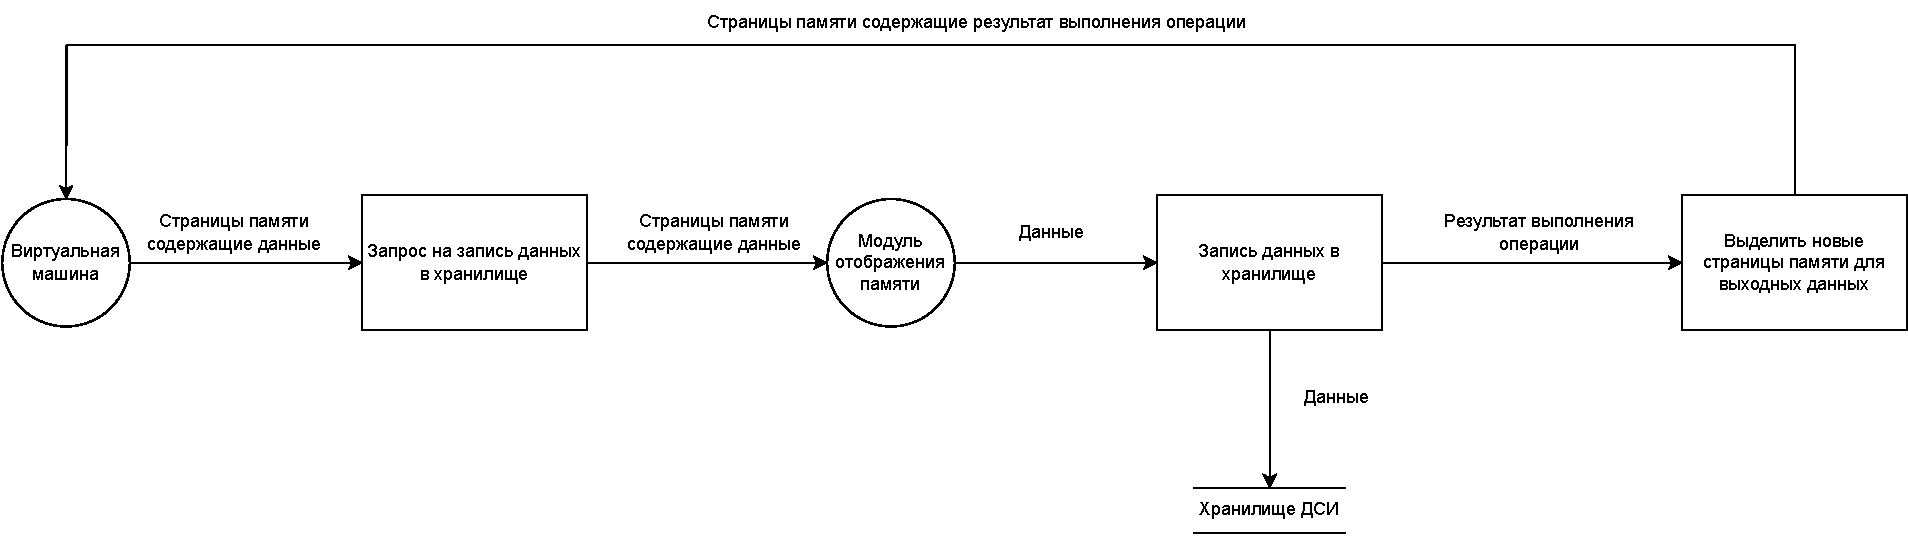
\includegraphics[width=\textwidth]{img/dfd-ciee.pdf}
	\caption{Диаграмма потоков данных операции записи в хранилище рабочего окружения}
	\label{fig:ciee}
\end{figure}

\subsection{Формализованное описание метода}

Разрабатываемый метод -- это виртуализация механизмов защиты, которые предоставляет аппаратная реализация ДСИ ARM TrustZone. На рисунках \ref{fig:idef0-main-1} - \ref{fig:idef0-main-2} представлена IDEF0-диаграмма и её детализированная версия метода программной реализации доверенной среды исполнения с помощью виртуализации процессоров архитектуры ARM. В следующих разделах будет представлено более подробное описание механизмов представленных на рисунке \ref{fig:idef0-main-2}.

\begin{figure}[h]
	\centering
	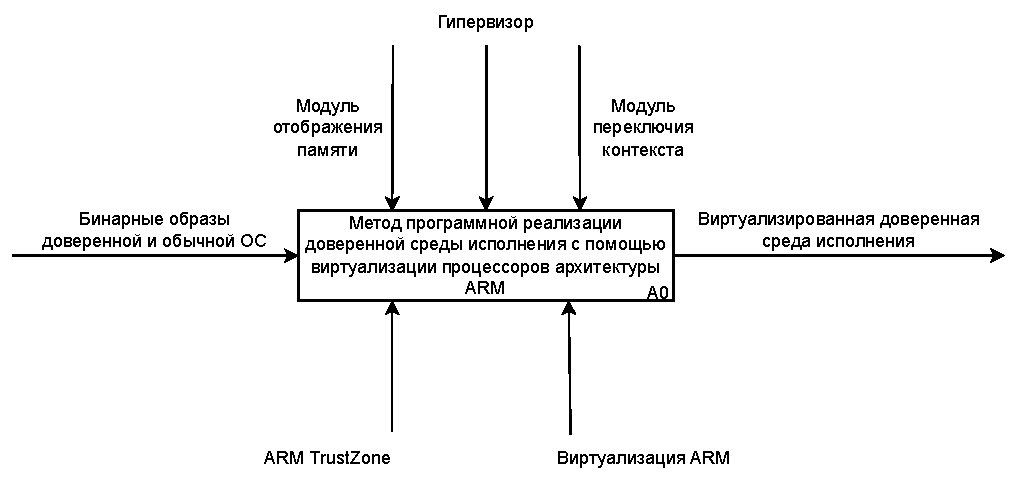
\includegraphics[width=\textwidth]{img/main-idef0-1.pdf}
	\caption{IDEF0-диаграмма разработанного метода}
	\label{fig:idef0-main-1}
\end{figure}

\begin{figure}[h]
	\centering
	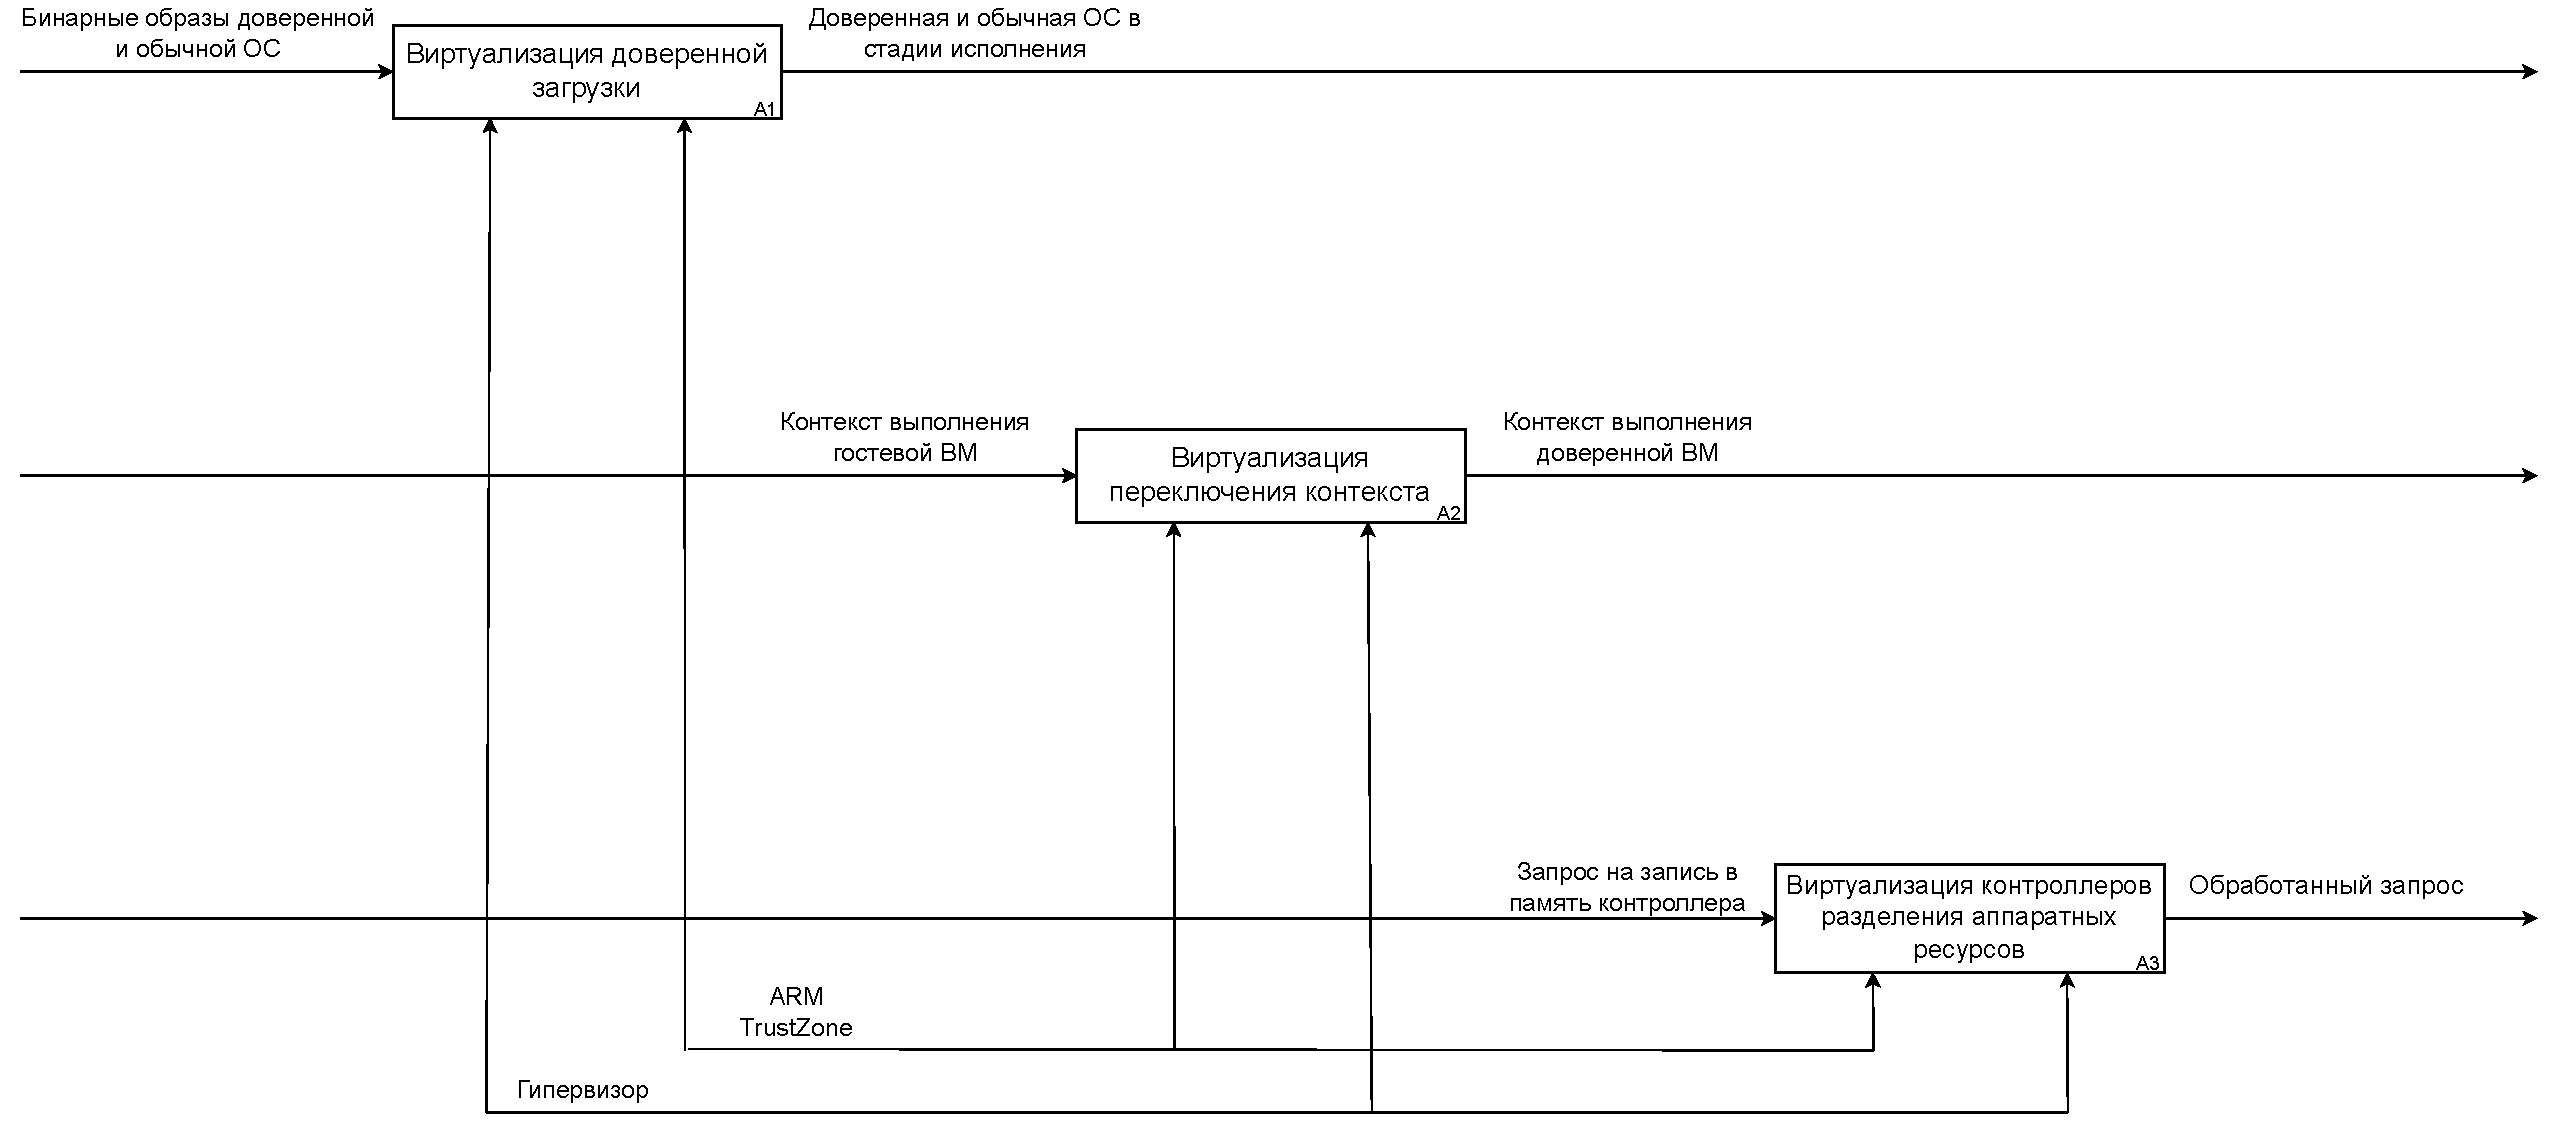
\includegraphics[width=\textwidth]{img/main-idef0-2.pdf}
	\caption{Детализированная IDEF0-диаграмма разработанного метода}
	\label{fig:idef0-main-2}
\end{figure}

\subsubsection{Описание доверенной загрузки}

Доверенная загрузка используется для обеспечения целостности загрузки системы. Процесс загрузки устройства с поддержкой ARM TrustZone включает в себя пять этапов.

\begin{itemize}
	\item [---] Загрузка загрузчика ОС из защищенного от воздействия внешних источников ПЗУ.
	\item [---] Инициализация окружения и загрузка ядра доверенной ОС.
	\item [---] Доверенное ядро инициализирует и настраивает окружение для корректной работы безопасного мира.
	\item [---] Доверенное ядро загружает в память загрузчик обычной ОС и передаёт ему управление.
	\item [---] Загрузчик обычной ОС вычисляет контрольную сумму бинарного образа ОС перед его загрузкой в память и загружает ОС.
\end{itemize}

Для виртуализации доверенной загрузки необходимо обеспечить следующие свойства:

\begin{enumerate}
	\item ядро доверенной ОС должно загрузиться до загрузки обычного;
	\item образ обычной ОС должен быть проверен;
	\item образ ОС не может быть подменён.
\end{enumerate}

На рисунке \ref{fig:idef0-secure-boot-2} представлена детализированная IDEF0-диаграмма виртуализации доверенной загрузки. Данная схема полностью удовлетворяет свойствам, которые были описаны выше.

\begin{figure}[h]
	\centering
	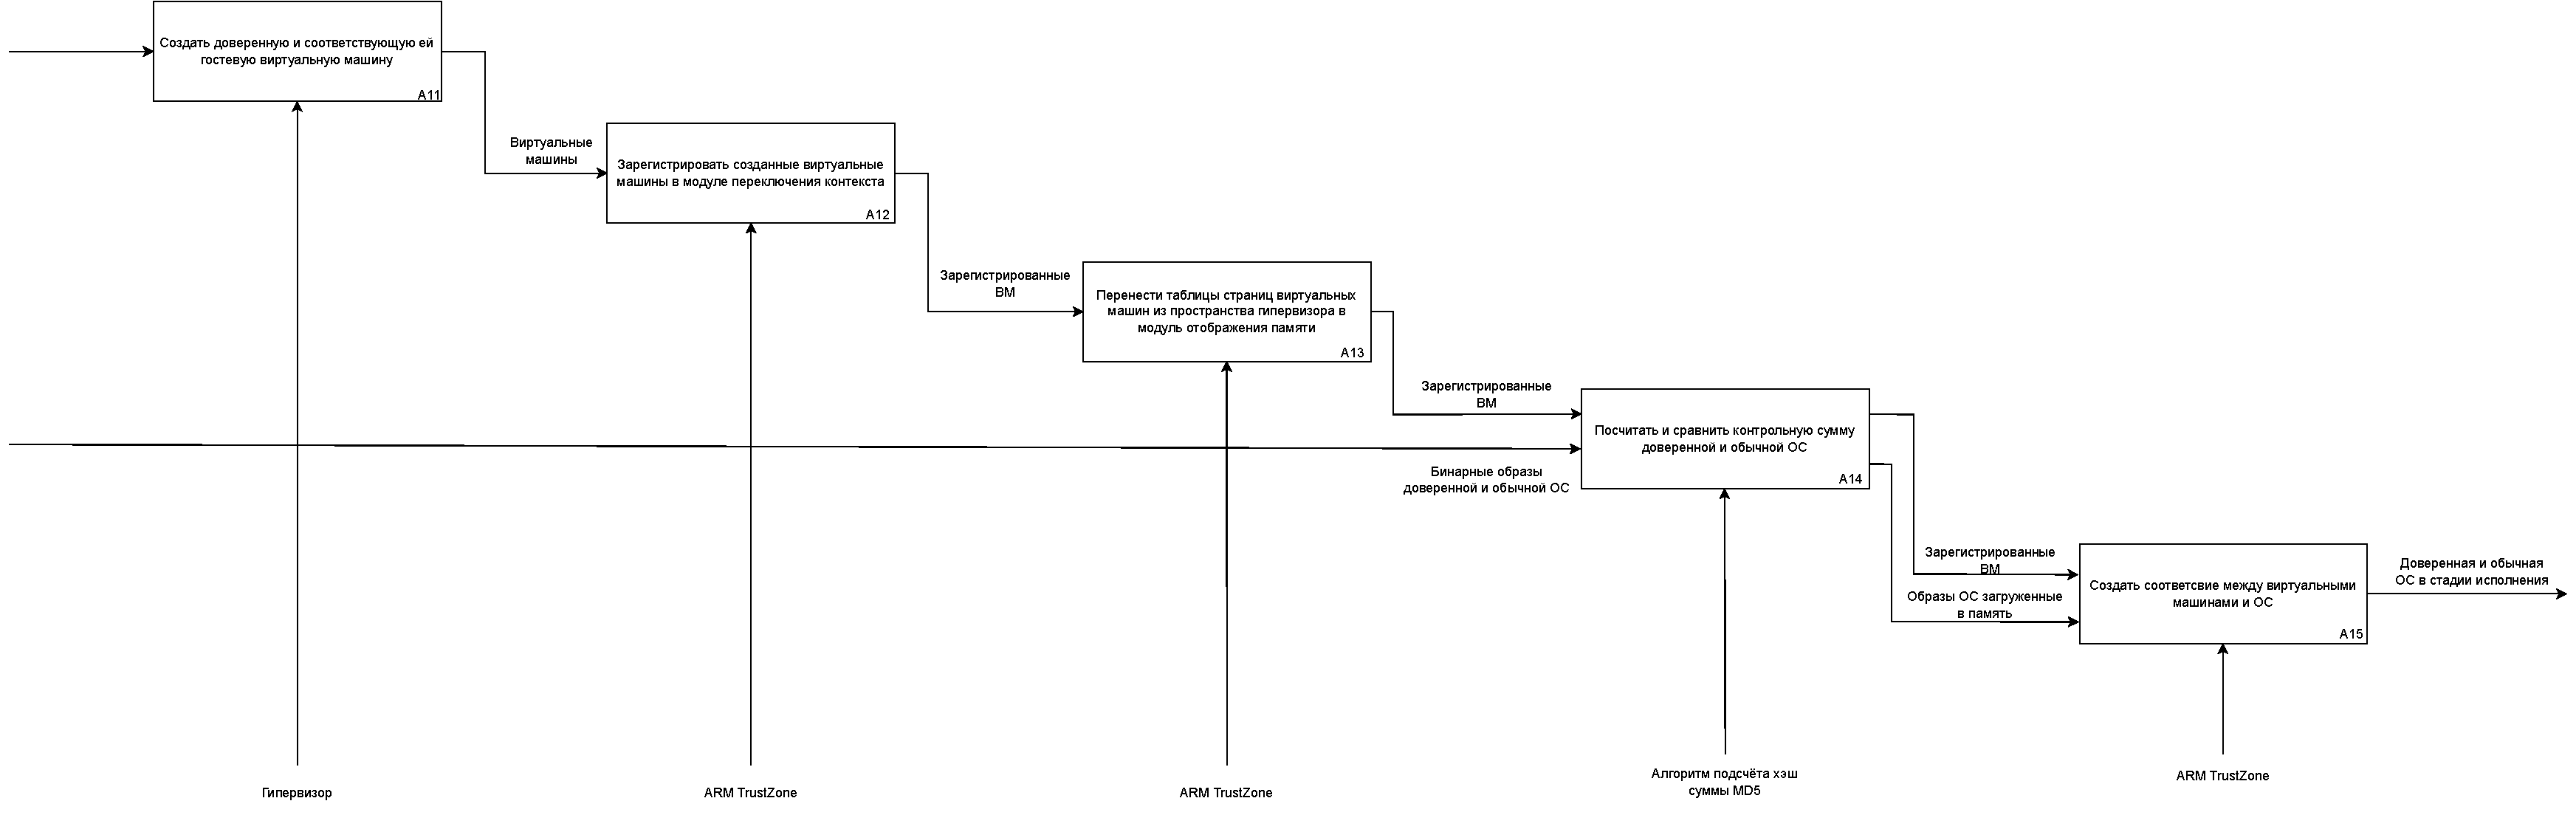
\includegraphics[width=\textwidth]{img/idef0-secure-boot-2.pdf}
	\caption{Детализированная IDEF0-диаграмма виртуализации доверенной загрузки}
	\label{fig:idef0-secure-boot-2}
\end{figure}

На рисунке \ref{fig:move-pte-algo} представлена схема алгоритма регистрации виртуальных машин в безопасном мире (в модуле переключения контекста).

\begin{figure}[h]
	\centering
	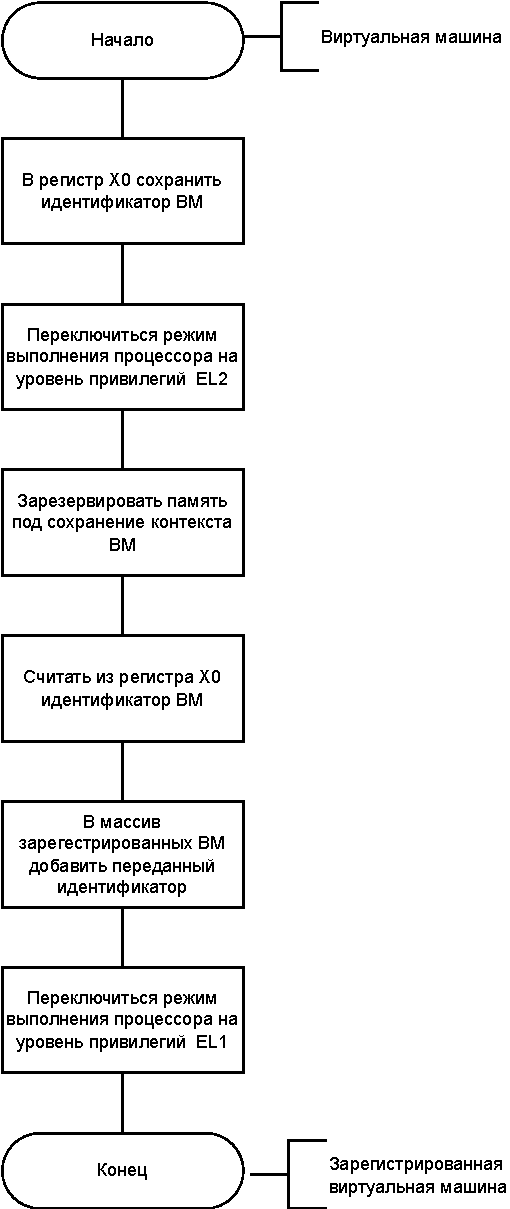
\includegraphics[scale=0.6]{img/register-vm-algo.pdf}
	\caption{Схема алгоритма регистрации виртуальных машин в безопасном мире}
	\label{fig:move-pte-algo}
\end{figure}

\subsubsection{Описание защиты и переключение контекста выполнения}

Каждый из миров (безопасный и обычный) имеют свой контекст выполнения -- значения регистров, настройка памяти, структуры данных и так далее. Реализация ARM TrustZone предоставляет функциональности защиты этого контекста -- каждый контекст доступен для чтения и записи только из мира, к которому он принадлежит.

На рисунке \ref{fig:idef0-context-switch-2} представлена детализированная IDEF0-диаграмма виртуализации переключения контекста между гостевой виртуальной машиной и доверенной. Контекст выполнения остаётся защищенным, т.к. сохраняется и восстанавливается он из безопасного мира. Обратная схема переключения контекста (из доверенной в гостевую ВМ) аналогична.

\begin{figure}[h]
	\centering
	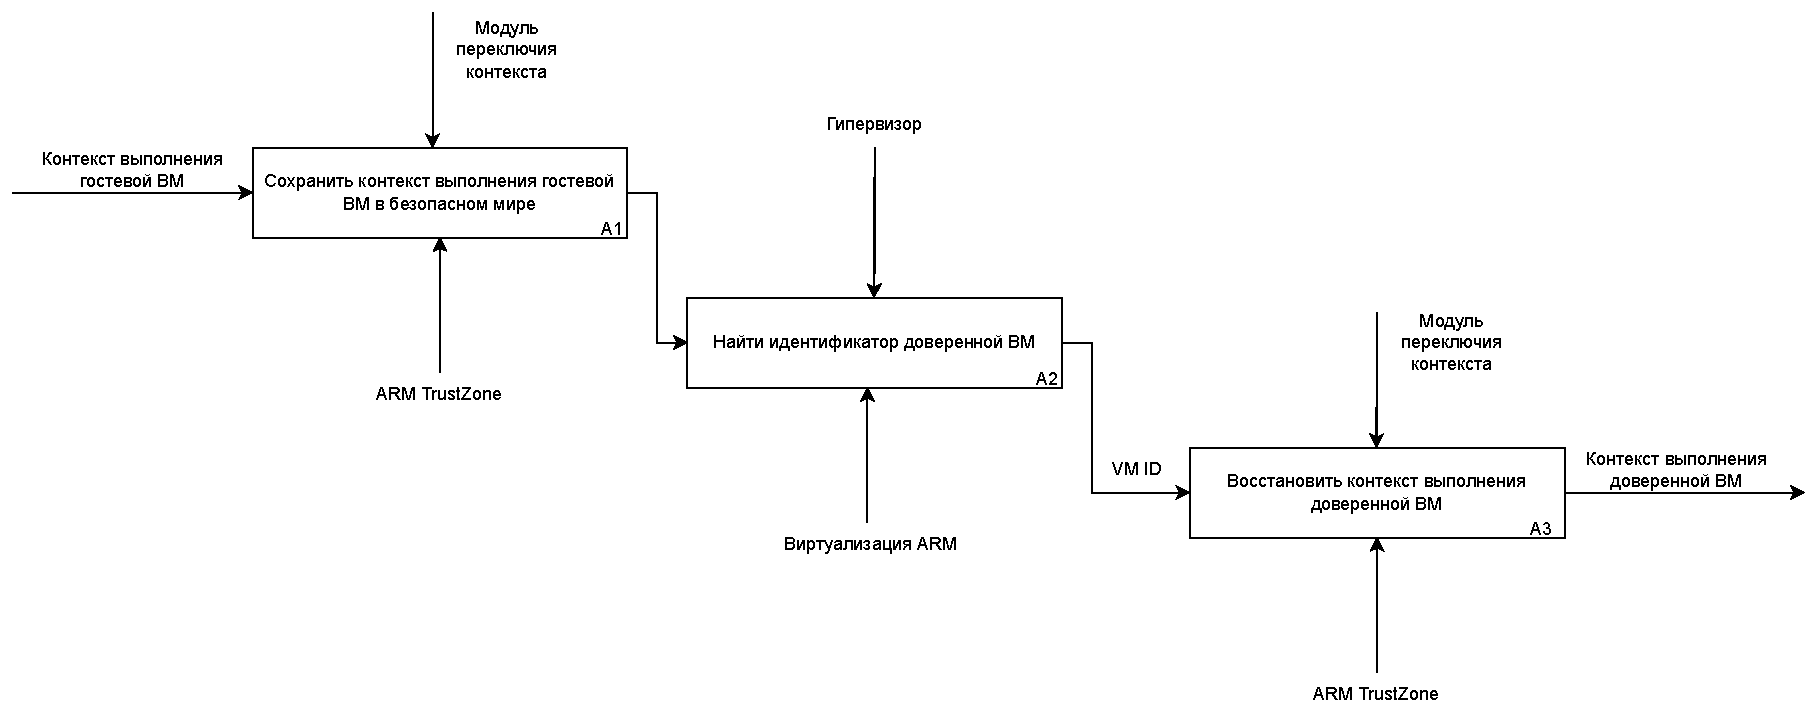
\includegraphics[width=\textwidth]{img/idef0-context-switch-2.pdf}
	\caption{Детализированная IDEF0-диаграмма виртуализации переключения контекста}
	\label{fig:idef0-context-switch-2}
\end{figure}

На рисунке \ref{fig:save-context-algo} представлена схема алгоритма сохранения контекста выполнения виртуальной машины в безопасном мире.

\begin{figure}[h]
	\centering
	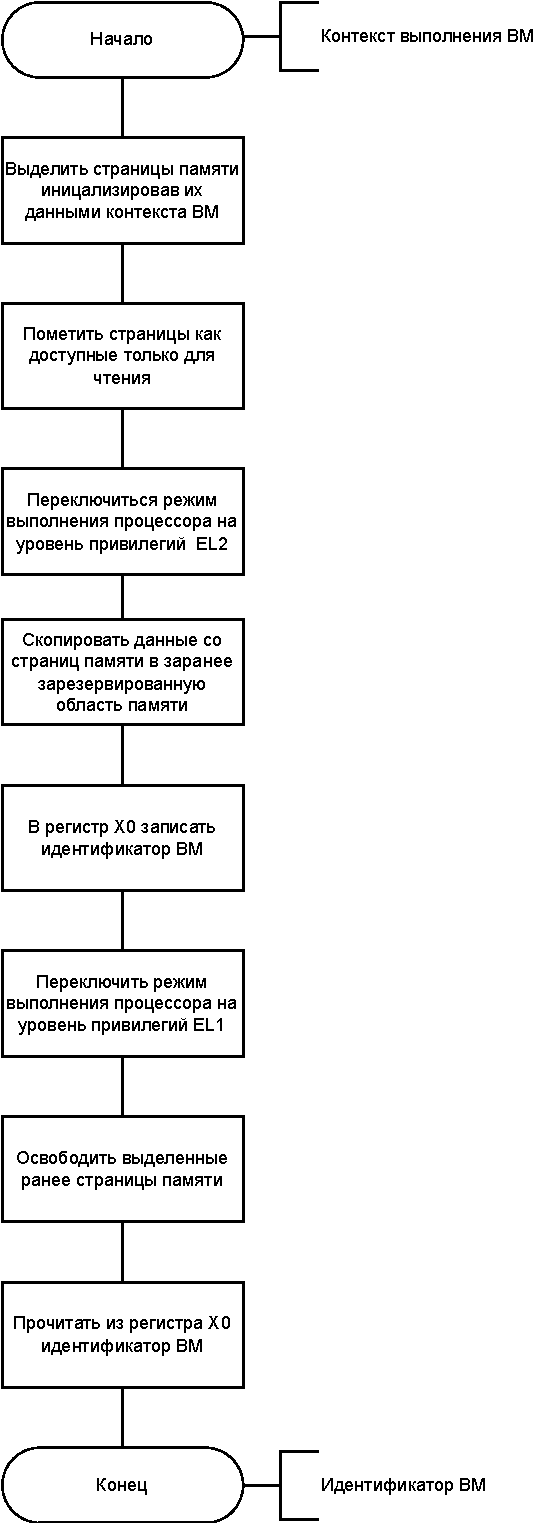
\includegraphics[scale=0.6]{img/save-context-algo.pdf}
	\caption{Схема алгоритма контекста выполнения виртуальной машины}
	\label{fig:save-context-algo}
\end{figure}

\subsubsection{Описание разделения аппаратных ресурсов}

ARM TrustZone разделяет аппаратные ресурсы (память, периферия, прерывания) между безопасным и обычном миром. Для каждого из этих ресурсов существует отдельный контроллер, который отвечает за их настройку и распределение между мирами. Все три контроллера могут быть настроены только из безопасного мира. Таким образом, необходимо виртуализировать каждый их этих контроллеров.

Для каждой виртуальной машины область памяти в которой находятся контроллеры помечена как только для чтения. В результате попытки записи в эти контроллеры, процессор вызывает исключение и управление передаётся гипервизору для его дальнейшей обработки. Такой подход называется trap-and-emulate \cite{trap-and-emulate}. 

На рисунке \ref{fig:idef0-trap-and-emulate-2} представлена детализированная IDEF0-диаграмма виртуализации контроллеров разделения аппаратных ресурсов. 

\begin{figure}[h]
	\centering
	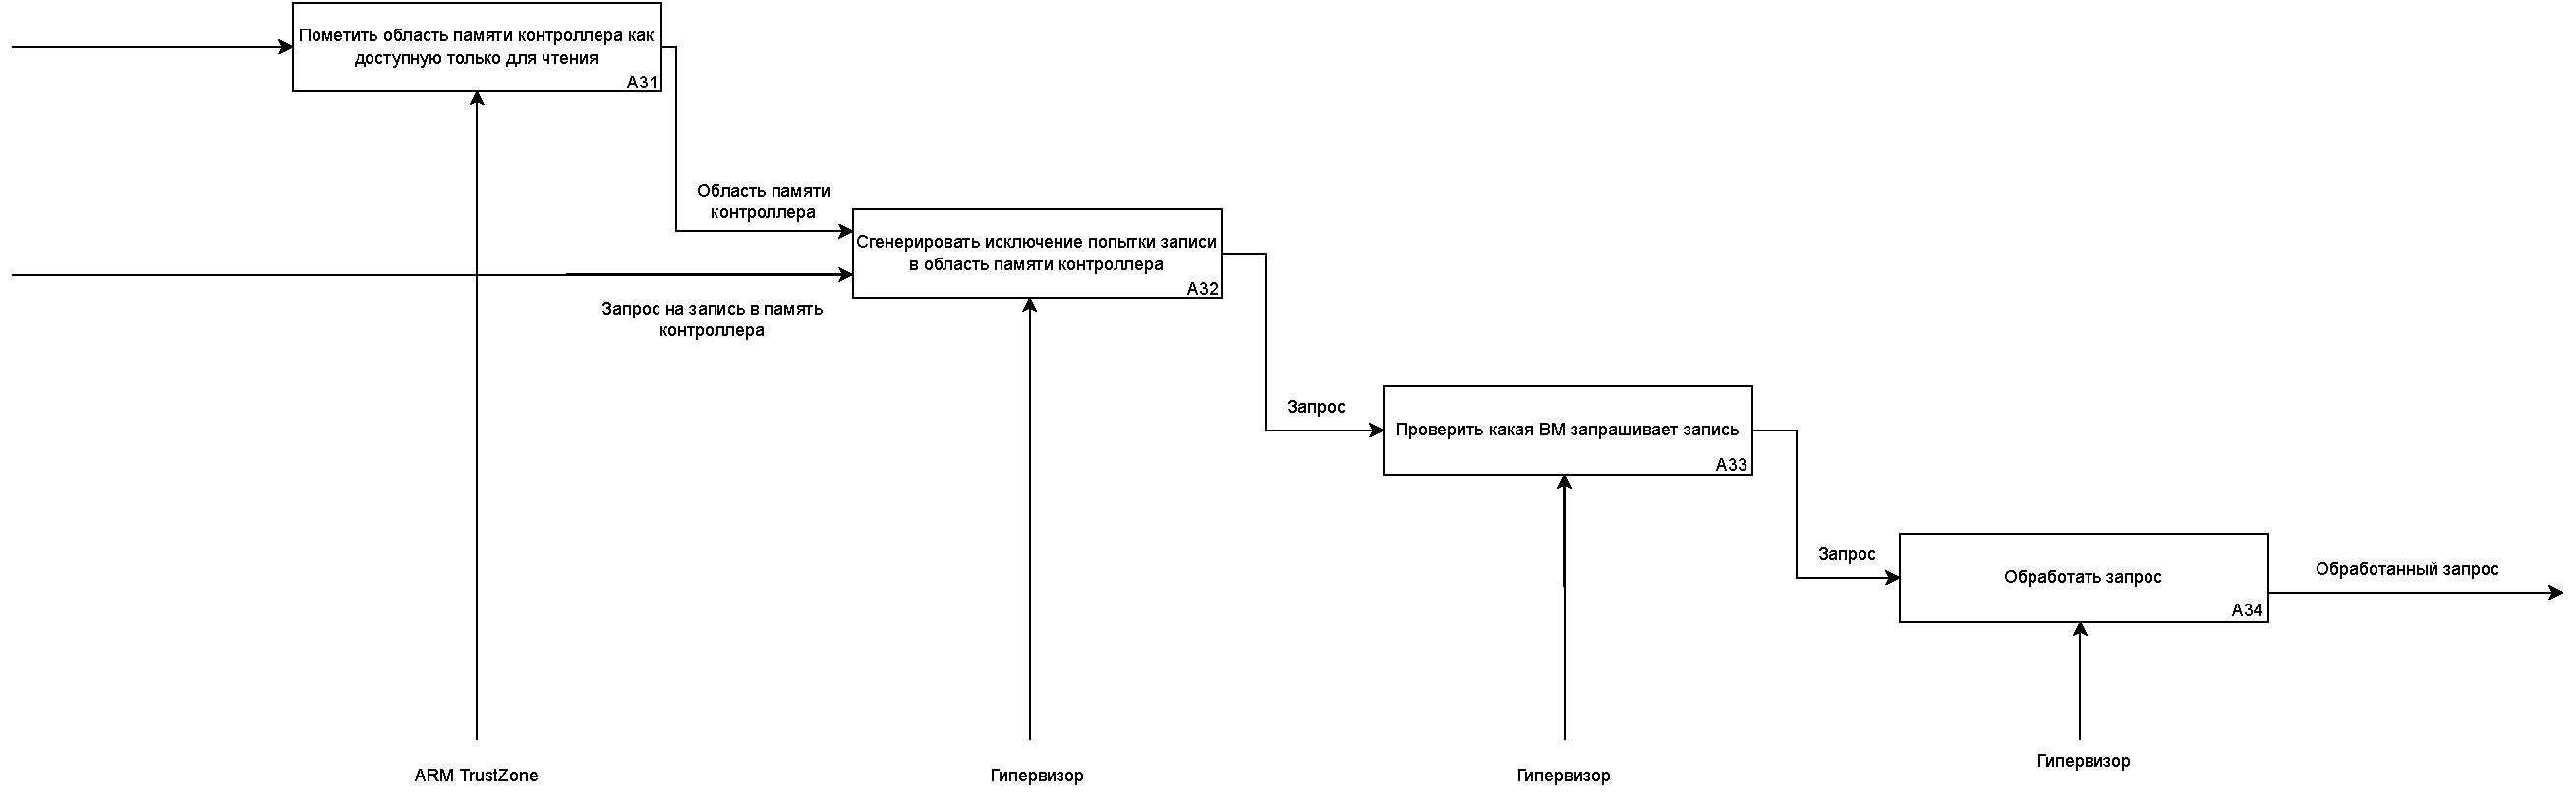
\includegraphics[width=\textwidth]{img/idef0-trap-and-emulate-2.pdf}
	\caption{Детализированная IDEF0-диаграмма виртуализации контроллеров разделения аппаратных ресурсов}
	\label{fig:idef0-trap-and-emulate-2}
\end{figure}

\subsection*{Вывод}

Был разработан метод программной реализации доверенной среды исполнения с помощью виртуализации процессоров архитектуры ARM. Были спроектированы и разработаны следующие компоненты:

\begin{itemize}
	\item модуль защищенного отображения памяти;
	\item модуль блокировки потока управления;
	\item модуль переключения контекста;
	\item индивидуальное рабочее окружение.
\end{itemize}
 
Представлено формализованное описание метода в виде IDEF0-диаграммы, состоящей из трех уровней, которые так же были детализированы:

\begin{itemize}
	\item виртуализация доверенной загрузки;
	\item виртуализация переключения контекста;
	\item виртуализация контроллеров разделения аппаратных ресурсов.
\end{itemize}

С помощью схем алгоритмов описаны используемые в разработанном методе алгоритмы:

\begin{itemize}
	\item регистрация виртуальных машин в безопасном мире;
	\item сохранение контекста выполнения виртуальной машины.
\end{itemize}

\pagebreak
